\section{Graphs}

\paragraph{}
The definitions are inspired by~\cite{diestel2017graph}

\begin{definition}[Graph]\index{graph}\index{vertex}\index{edge}
  A \textit{graph} is a pair $G = (V, E)$ of sets such that $E \subseteq V \times V$. The elements of $V$ are called \textit{vertices} and the elements of $E$ are called \textit{edges}.
\end{definition}

\begin{definition}[Undirected graph]\index{undirected graph}
  A graph $G = (V,E)$ is \textit{undirected} if $(a,b) \in V \Leftrightarrow (b,a) \in V$.
\end{definition}

\paragraph{}
In general all graphs are supposed to be undirected if not otherwise stated.

\paragraph{}
Graphs are often represented as drawing.  Each vertex is represented by a dot. An edge is represented by a line between the two dots that compose it.

\paragraph{}
For example, a graph with $V = \{1,2,3,4\}$ and $E = \{(1,2), (2,3), (3,4), (1,3)\}$ can be drawn as this:

\begin{figure}[H]
  \begin{center}
    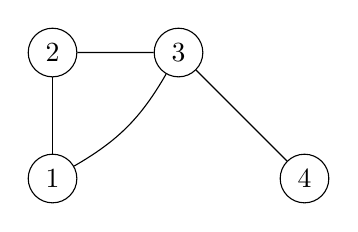
\begin{tikzpicture}[scale=.8]

      \begin{scope}[every node/.style={circle,draw}]
        \node (1)  at (0,0) {1};
        \node (2)  at (0,2) {2};
        \node (3)  at (2,2) {3};
        \node (4)  at (4,0) {4};
      \end{scope}


      \begin{scope}[every edge/.style={draw}]
        \path (1)  edge node {} (2);
        \path (2)  edge node {} (3);
        \path (3)  edge[bend left=15] node {} (1);
        \path (3)  edge node {} (4);
      \end{scope}

    \end{tikzpicture}
    \caption{Example of a representation of a graph}
  \end{center}
\end{figure}

\paragraph{}
The drawing of a graph is obviously not unique.

\paragraph{}
When not needed the numbers on the graphs are often removed.


\begin{figure}[H]
  \begin{center}
    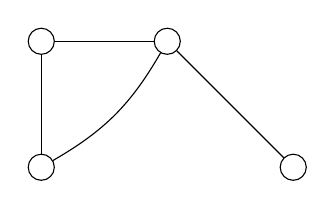
\begin{tikzpicture}[scale=.8]

      \begin{scope}[every node/.style={circle,draw}]
        \node (1)  at (0,0) {};
        \node (2)  at (0,2) {};
        \node (3)  at (2,2) {};
        \node (4)  at (4,0) {};
      \end{scope}


      \begin{scope}[every edge/.style={draw}]
        \path (1)  edge node {} (2);
        \path (2)  edge node {} (3);
        \path (3)  edge[bend left=15] node {} (1);
        \path (3)  edge node {} (4);
      \end{scope}

    \end{tikzpicture}
    \caption{Example of a representation of a graph}
  \end{center}
\end{figure}

\begin{definition}[Labeled graph]\index{labeled graph}
  A labeled graph is a graph where the vertices are not just only in $V \times V$ but in $V \times V \times L$ where $L$ is a finite set of labels.
\end{definition}

\paragraph{}
When we draw a labeled graph we write the label on the edge.

\begin{figure}[H]
  \begin{center}
    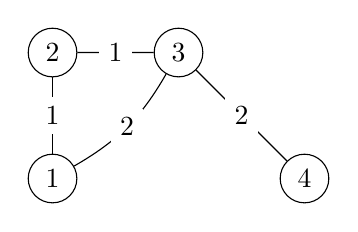
\begin{tikzpicture}[scale=.8]

      \begin{scope}[every node/.style={circle,draw}]
        \node (1)  at (0,0) {1};
        \node (2)  at (0,2) {2};
        \node (3)  at (2,2) {3};
        \node (4)  at (4,0) {4};
      \end{scope}

      \begin{scope}[every node/.style={fill=white}]
        \begin{scope}[every edge/.style={draw}]
          \path (1)  edge node {1} (2);
          \path (2)  edge node {1} (3);
          \path (3)  edge[bend left=15] node {2} (1);
          \path (3)  edge node {2} (4);
        \end{scope}
      \end{scope}

    \end{tikzpicture}
    \caption{Example of a labeled graph}
  \end{center}
\end{figure}

\begin{definition}[Multigraph]\index{multigraph}
  A multigraph is a graph where two vertices can be linked multiples times
\end{definition}

\begin{figure}[H]
  \begin{center}
    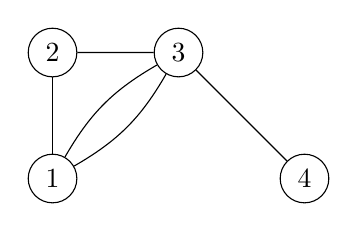
\begin{tikzpicture}[scale=.8]

      \begin{scope}[every node/.style={circle,draw}]
        \node (1)  at (0,0) {1};
        \node (2)  at (0,2) {2};
        \node (3)  at (2,2) {3};
        \node (4)  at (4,0) {4};
      \end{scope}


      \begin{scope}[every edge/.style={draw}]
        \path (1)  edge node {} (2);
        \path (2)  edge node {} (3);
        \path (3)  edge[bend left=15] node {} (1);
        \path (3)  edge[bend right=15] node {} (1);
        \path (3)  edge node {} (4);
      \end{scope}

    \end{tikzpicture}
    \caption{Example of a multigraph}
  \end{center}
\end{figure}

\paragraph{}
It is possible to define a multigraph with labels.

\begin{definition}[Isomorphism of graph]
  Two graphs are isomorphic if it exists a bijection between the vertices of the two graphs such that....
\end{definition}
